%-------------------------------------------------------------------------------
\chapter{Joint limits}
\label{app.jointconstraints}
\acresetall
%-------------------------------------------------------------------------------

%%%%%%%%%%%%%%%%%%%%%%%%%%%%%%%%%%%%%%%%%%%%%%%%%%%%%%%%%%%%%%%%%%%%%%%%%%%%%%%%
%%%%%%%%%%%%%%%%%%%%%%%%%%%%%%%%%%%%%%%%%%%%%%%%%%%%%%%%%%%%%%%%%%%%%%%%%%%%%%%%
%%%%%%%%%%%%%%%%%%%%%%%%%%%%%%%%%%%%%%%%%%%%%%%%%%%%%%%%%%%%%%%%%%%%%%%%%%%%%%%%
\section{Bounds on the joint angular accelerations}

Joint angles $\qn$ and angular velocities $\dqn$ are parts of the state of the
whole body model considered in \cref{sec.whole_body_model}, while joint angular
accelerations $\ddqn$ are controlled variables. When the whole body model is
used for instantaneous control of the robot, it is not possible to constrain
$\qn$ and $\dqn$ directly, but we can constrain $\qn_{T}$ and $\dqn_{T}$
%
\begin{align}
    &\qn_{T} = \qn + T \dqn + \frac{T^2}{2} \ddqn,\\
    &\dqn_{T} = \dqn + T \ddqn,
\end{align}
%
which will be reached in time $T$ starting from the current time instant
assuming constant $\ddqn$ on $[0,T]$ \cite{Rubrecht2012auro, Saab2013tro}.
Moreover, the joint bounds may conflict with each other: when a joint hits its
mechanical limit, there is no guarantee that bounds on angular velocities and
accelerations are respected. We resolve the conflicts by introducing
prioritization (see \cref{ch.optimization}) of the bounds
%
\begin{hierarchy}[hr.joints_bounds]
    \level $\ubar{\q}^{\prime}  \le  \qn_{T}  \le  \bar{\q}^{\prime}$
    \level $\ubar{\dq}^{\prime}  \le  \dqn_{T}  \le  \bar{\dq}^{\prime}$
    \level $\ubar{\ddq}^{\prime}  \le  \ddqn  \le  \bar{\ddq}^{\prime}$
\end{hierarchy}
%
so that the position limits take over the velocity and acceleration limits.


All constraints in \cref{hr.joints_bounds} are expressed as bounds on $\ddqn$
%
\begin{hierarchy}[hr.joints_bounds_acc]
    \level $\ubar{\q}\vphantom{q}^{\prime}_{p}  \le  \ddqn  \le  \bar{\q}\vphantom{q}^{\prime}_{p}$
    \level $\ubar{\q}\vphantom{q}^{\prime}_{v} \le  \ddqn  \le  \bar{\q}\vphantom{q}^{\prime}_{v}$
    \level $\ubar{\ddq}\vphantom{q}^{\prime}        \le  \ddqn  \le  \bar{\ddq}\vphantom{q}^{\prime}$
\end{hierarchy}
%
where
%
\begin{subequations}
    \begin{align}
        \ubar{\q}\vphantom{q}^{\prime}_{p}
        =
        \frac{2\left(\ubar{\q}^{\prime} - \qn\right)}{T^2} - \frac{2 \dqn}{T}
        &,
        \quad
        \bar{\q}\vphantom{q}^{\prime}_{p}
        =
        \frac{2\left(\bar{\q}^{\prime} - \qn\right)}{T^2} - \frac{2 \dqn}{T},
        \label{eq.bad_joint_bounds}
        \\
        \ubar{\q}\vphantom{q}^{\prime}_{v}
        =
        \frac{\left(\ubar{\dq}^{\prime} - \dqn \right)}{T}
        &,
        \quad
        \bar{\q}\vphantom{q}^{\prime}_{v}
        =
        \frac{\left(\bar{\dq}^{\prime} - \dqn \right)}{T}
        ,
    \end{align}
\end{subequations}
%
and division by $T$ is safe, since it is always greater than zero. Constraints
in \cref{hr.joints_bounds_acc} are redundant and are preprocessed to collapse
it to a single level and reduce the number of constraints 3 times.


Computation of $\ubar{\q}\vphantom{q}^{\prime}_{p}$ and
$\bar{\q}\vphantom{q}^{\prime}_{p}$ as suggested in \cref{eq.bad_joint_bounds}
is potentially unsafe and we construct them using a slightly different approach
described in the following section.



%%%%%%%%%%%%%%%%%%%%%%%%%%%%%%%%%%%%%%%%%%%%%%%%%%%%%%%%%%%%%%%%%%%%%%%%%%%%%%%%
%%%%%%%%%%%%%%%%%%%%%%%%%%%%%%%%%%%%%%%%%%%%%%%%%%%%%%%%%%%%%%%%%%%%%%%%%%%%%%%%
%%%%%%%%%%%%%%%%%%%%%%%%%%%%%%%%%%%%%%%%%%%%%%%%%%%%%%%%%%%%%%%%%%%%%%%%%%%%%%%%
\section{Bounds on the joint angles}

\begin{figure}[ht]
    \begin{minipage}[t]{0.45\textwidth}
        \centering{%
        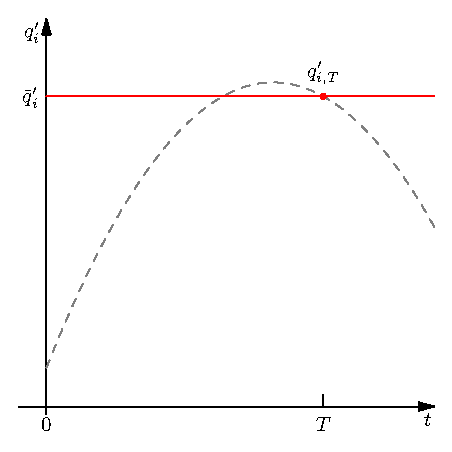
\includegraphics{joint_bound_bad.eps}}
        \subcaption{
            Violation of the upper bound of $i$-th joint angle. Solid red line
            and dashed grey curve indicate the bound the joint angle
            trajectory.
        }
        \label{fig.joint_bound_bad}
    \end{minipage}
    \hfill
    \begin{minipage}[t]{0.45\textwidth}
        \centering{%
        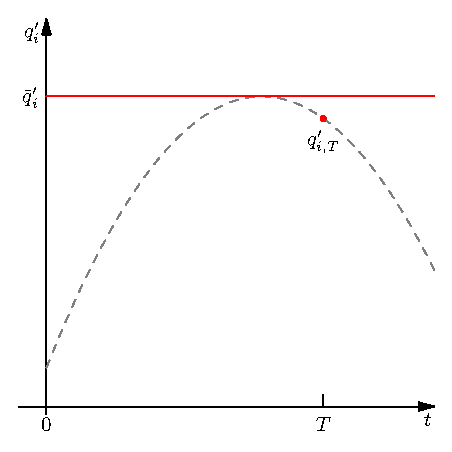
\includegraphics{joint_bound_good.eps}}
        \subcaption{
            All values of $i$-th joint angle in the time interval $[0,T]$ lie
            below the upper bound.
        }
        \label{fig.joint_bound_good}
    \end{minipage}
    \caption[Respecting the upper bound of the $i$-th joint angle.]{
        Respecting the upper bound of the $i$-th joint angle.
    }
    \label{fig.joint_bound}
\end{figure}


Note that the bounds \cref{eq.bad_joint_bounds} are quadratic in
$1/T$, which means that satisfaction of $\ubar{\q}^{\prime}  \le
\qn_{T} \le  \bar{\q}^{\prime}$ does not imply satisfaction $\ubar{\q}^{\prime}
\le  \qn_{t}  \le \bar{\q}^{\prime}$ for $t \in (0, T)$ as illustrated in
\cref{fig.joint_bound_bad}. In practice, imposing only $\ubar{\q}^{\prime}  \le
\qn_{T} \le \bar{\q}^{\prime}$ results in violations of the joint bounds in the
model and collisions in the joints of the robot. However, this issue can be
avoided by exploiting the quadratic nature of the constraint.


Let us substitute variable $\nu = \frac{1}{t}$ with $t \in (0, T]$ into the
upper bound on acceleration of $i$-th joint $\ddqni$
%
\begin{equation}\label{eq.upper_bound_i}
    \bar{q}\vphantom{q}^{\prime}_{p,i}
    =
    2 \left(\bar{q}\vphantom{q}^{\prime}_i - \qni \right) \nu^2 - 2 \dqni \nu.
\end{equation}
%
Then in order to make sure that the joint angle constraint is not violated for
all $t \in (0, T]$ as shown in \cref{fig.joint_bound_good}, we have to make
sure that $\ddqni$ does not exceed the minimal value of
\cref{eq.upper_bound_i}. The minimal value is obtained by solving the following
\ac{QP}
%
\begin{equation}
    \begin{aligned}
        \MINIMIZE{\nu}  & 2 \left(\bar{q}^{\prime}_i - \qni \right) \nu^2 - 2 \dqni \nu \\
        \SUBJECTTO      & \nu \ge \frac{1}{T}.
    \end{aligned}
\end{equation}
%


Solution $\nu^{\star}$ of this \ac{QP} is unbounded in two cases
%
\begin{itemize}
    \item when $\bar{q}^{\prime}_i < \qni$, \IE, the bound is already violated;
    \item when $\bar{q}^{\prime}_i = \qni$ and $\dqni > 0$, \IE, the bound
        is reached with non-zero velocity.
\end{itemize}
%
The first case corresponds to a situation when there is a mismatch between the
state of the model and the robot, since the physical constraint cannot be
violated. In the second case there is an inevitable collision in the joint.
Such collisions can be simulated using an impact law similar to the one
described in \cref{app.collision}, but validity of such simulation is
questionable without an accurate joint model. Thus, in both cases there is no
$\ddqni$, which prevents violation of the bound or collision with it. One
possible approach to recover from such situations is to assume $\nu^{\star} =
\frac{1}{T}$. Neither of these cases, however, was observed in our simulations.


When the solution $\nu^{\star}$ is bounded, it coincides with extremum of the
objective function or the bound $1/T$:
%
\begin{equation}
    \nu^{\star} =
    \left\{
    \begin{aligned}
        &\frac{\dqni}{2 \left(\bar{q}^{\prime}_i - \qni \right)},
        \quad
        &&
        \mbox{if}
        \quad
        \bar{q}^{\prime}_i > \qni
        \quad
        \mbox{and}
        \quad
        \frac{\dqni}{2 \left(\bar{q}^{\prime}_i - \qni \right)} \ge \frac{1}{T} \\
        &\frac{1}{T},
        \quad
        &&
        \mbox{otherwise.}
    \end{aligned}
    \right.
\end{equation}
%
The upper bound on $\ddqni$ is obtained by substitution of $\nu^{\star}$ in the
objective function and is equal to
%
\begin{equation}
    \bar{q}\vphantom{q}^{\prime}_{p,i}
    =
    \left\{
        \begin{aligned}
            &- \frac{(\dqni)^2}{2 \left(\bar{q}^{\prime}_i - \qni \right)},
            \quad
            &&
            \mbox{if}
            \quad
            \bar{q}^{\prime}_i > \qni
            \quad
            \mbox{and}
            \quad
            \frac{\dqni}{2 \left(\bar{q}^{\prime}_i - \qni \right)} > \frac{1}{T}
            \\
            &
            \frac{2\left(\bar{q}^{\prime}_i - \qni \right)}{T^2} - \frac{2 \dqni}{T},
            \quad
            &&
            \mbox{otherwise.}
        \end{aligned}
    \right.
\end{equation}
%
The lower bound on acceleration is determined equivalently by solving a
maximization problem. There exist a possibility of conflict between the lower
and upper bounds, \IE, $\bar{q}\vphantom{q}^{\prime}_{p,i} <
\ubar{q}\vphantom{q}^{\prime}_{p,i}$, if the joint angular velocity is high,
but we did not observe such situations in our simulations.


%%%%%%%%%%%%%%%%%%%%%%%%%%%%%%%%%%%%%%%%%%%%%%%%%%%%%%%%%%%%%%%%%%%%%%%%%%%%%%%%
%%%%%%%%%%%%%%%%%%%%%%%%%%%%%%%%%%%%%%%%%%%%%%%%%%%%%%%%%%%%%%%%%%%%%%%%%%%%%%%%
%%%%%%%%%%%%%%%%%%%%%%%%%%%%%%%%%%%%%%%%%%%%%%%%%%%%%%%%%%%%%%%%%%%%%%%%%%%%%%%%
\section{Imposing position constraints through accelerations}

So far we were considering bounds on the joint angles, but sometimes general
constraints on position such as
%
\begin{equation}\label{eq.general_ctr_acc}
    \ubar{b}_{\V{y}} \le \M{A} \V{y} \le \bar{b}_{\V{y}}
\end{equation}
%
with $\V{y} \in \RR^p$ and $\M{A} \in \RR^{1 \CROSS p}$ must also be ensured
using constraints on acceleration
%
\begin{equation}
    \ubar{b}_{\ddotV{y}} \le \M{A} \ddotV{y} \le \bar{b}_{\ddotV{y}}.
\end{equation}
%
For example, we might be interested in constraining projection of the \ac{CoM}
position to support area using acceleration of the \ac{CoM}. In this case, the
upper bound $\bar{b}_{\ddotV{y}}$ is
%
\begin{equation}
    \bar{b}_{\ddotV{y}}
    =
    \left\{
    \begin{aligned}
        & - \frac{(\M{A}\dotV{y})^2}{2\left(\bar{b}_{\V{y}} - \M{A}\V{y}\right)}
            \quad &&\mbox{if} \quad
            \ubar{b}_{\V{y}} - \M{A}\V{y} > 0
            \quad \mbox{and} \quad
            \frac{\M{A}\dotV{y}}{2\left(\bar{b}_{\V{y}} - \M{A}\V{y}\right)} > \frac{1}{T} \\
        &   \frac{2 \left(\bar{b}_{\V{y}} - \M{A}\V{y}\right)}{T^2}  -  \frac{2 \M{A} \dotV{y}}{T}, \quad && \mbox{otherwise.}
    \end{aligned}
    \right.
\end{equation}
%
$\ubar{b}_{\ddotV{y}}$ is computed in a similar way.
